% !TeX root = slides.tex
\section{Probability Distributions}

\subsection{Recommended References}
\begin{frame}{Probability Distributions - Recommended References}
	\begin{vfilleditems}
		\item \textcite{grimmettProbabilityRandomProcesses2020}
		\begin{vfilleditems}
			\item Chapter 3: Discrete random variables
			\item Chapter 4: Continuous random variables
		\end{vfilleditems}
		\item \textcite{dekkingModernIntroductionProbability2010}
		\begin{vfilleditems}
			\item Chapter 4: Discrete random variables
			\item Chapter 5: Continuous random variables
		\end{vfilleditems}
		\item \textcite{betancourtProbabilisticBuildingBlocks2019}
	\end{vfilleditems}
\end{frame}

%--- Intro -----------------------------------------------------------%
\begin{frame}{Probability Distributions}
	Bayesian statistics uses probability distributions as the inference
	engine of the parameter and uncertainty estimates.
	\vfill
	Imagine that probability distributions are small ``Lego'' pieces.
	We can construct anything we want with these little pieces.
	We can make a castle, a house, a city; literally anything.
	The same is valid for Bayesian statistical models.
	We can construct models from the simplest ones to the most complex
	using probability distributions and their relationships.
\end{frame}

\begin{frame}
	\begin{defn}[Probability Distribution Function]
		A probability distribution function is a mathematical function
		that outputs the probabilities for different results of an
		experiment.
		It is a mathematical description of a random phenomena in terms
		of its sample space and the event probabilities (subsets
		of the sample space).
		$$P(X): X \to \mathbb{R} \in [0, 1]$$
		For discrete random variables, we define as ``mass'',
		and for continuous random variables, we define as ``density''.
	\end{defn}
\end{frame}

\begin{frame}{Mathematical Notation}
	We use the notation
	$$X \sim \text{Dist}(\theta_1, \theta_2, \dots)$$
	where:
	\begin{vfilleditems}
		\item $X$: random variable
		\item Dist: distribution name
		\item $\theta_1, \theta_2, \dots$: parameters that define how the
		distribution behaves
	\end{vfilleditems}
	Every probability distribution can be ``parameterized'' by specifying
	parameters that allow to control certain distribution aspects for
	a specific goal.
\end{frame}

\begin{frame}{Probability Distribution Function}
	\centering
	\begin{tikzpicture}
		\begin{axis}[every axis plot, line width=2pt,
				ylabel=PDF,
				xlabel={$X$},
				domain=-4:4,samples=200,
				axis x line*=bottom, % no box around the plot, only x and y axis
				axis y line*=left, % the * suppresses the arrow tips
				enlarge x limits=true, % extend the axes a bit
			]

			\addplot [blue] {gaussian(0, 1)};
		\end{axis}
	\end{tikzpicture}
\end{frame}

\begin{frame}
	\begin{defn}[Cumulative Distribution Function]
		The cumulative distribution function (CDF) of a random variable
		$X$ evaluated at $x$ is the probability that $X$ will take
		values less or qual than $x$:
		$$\text{CDF} = P(X \leq x)$$
	\end{defn}
\end{frame}

\begin{frame}{Cumulative Distribution Function}
	\centering
	\begin{tikzpicture}
		\begin{axis}[every axis plot, line width=2pt,
				ylabel=CDF,
				xlabel={$X$},
				domain=-4:4,samples=200,
				axis x line*=bottom, % no box around the plot, only x and y axis
				axis y line*=left, % the * suppresses the arrow tips
				enlarge x limits=true, % extend the axes a bit
			]

			\addplot [blue] {normcdf(0, 1)};
		\end{axis}
	\end{tikzpicture}
\end{frame}

%--- Discrete --------------------------------------------------------%
\subsection{Discrete Distributions}
\begin{frame}
	\begin{defn}[Discrete Distributions]
		Discrete probability distributions are distributions which the
		results are a discrete number:
		$-N, \dots, -2, 1, 0,1,2,\dots, N$ e $N \in \mathbb{Z}$.
		In discrete probability distributions we call the probability
		of a distribution taking certain values as ``mass''.
		The probability mass function (PMF) is the function that
		specifies the probability of a random variable $X$ taking value $x$:
		$$\text{PMF}(x) = P(X = x)$$
	\end{defn}
\end{frame}

\subsubsection{Discrete Uniform}
\begin{frame}{Discrete Uniform}
	The discrete uniform is a symmetric probability distribution in which
	a finite number of values are equally likely of being observable.
	Each one of the $n$ values have probability $\frac{1}{n}$.
	\vfill
	The uniform discrete distribution has two parameters and its notation is
	$\text{Uniform}(a, b)$:
	\begin{vfilleditems}
		\item $a$ -- lower bound
		\item $b$ -- upper bound
	\end{vfilleditems}
	\vfill
	Example: dice.
\end{frame}

\begin{frame}{Discrete Uniform}
	$$\text{Uniform}(a,b) = f(x, a, b) = \frac{1}{b-a+1} \text{ for $a \leq x \leq b$ and $x\in \{a,a+1,\dots ,b-1,b\}$}$$
\end{frame}

\begin{frame}{Discrete Uniform}
	\centering
	\begin{tikzpicture}
		\begin{axis}[every axis plot,
				ybar=0pt, bar width=0.3,
				ylabel=PMF,
				samples at={1,...,6}, % All plots: from 1:6, 6 samples only
				axis x line*=bottom, % no box around the plot, only x and y axis
				axis y line*=left, % the * suppresses the arrow tips
				enlarge x limits=true, % extend the axes a bit
			]

			\addplot [fill=blue] {discreteuniform(1, 6)};
			\addlegendentry{$a=1, b=6$}
		\end{axis}
	\end{tikzpicture}
\end{frame}

\subsubsection{Bernoulli}
\begin{frame}{Bernoulli}
	Bernoulli distribution describes a binary event of the success of an experiment.
	We represent $0$ as failure and $1$ as success, hence the result of a
	Bernoulli distribution is a binary variable $Y \in \{0, 1\}$.
	\vfill
	Bernoulli distribution is often used to model binary discrete results
	where there is only two possible results.
	\vfill
	Bernoulli distribution has only a single parameter and its notation is
	$\text{Bernoulli} (p)$:
	\begin{vfilleditems}
		\item $p$ -- probability of success
	\end{vfilleditems}
	\vfill
	Example: If the patient survived or died or if the client purchased or not.
\end{frame}

\begin{frame}{Bernoulli}
	$$\text{Bernoulli}(p) = f(x, p)=p^{x}(1-p)^{1-x} \text{ for $x \in \{0,1\}$}$$ %
\end{frame}

\begin{frame}{Bernoulli}
	\centering
	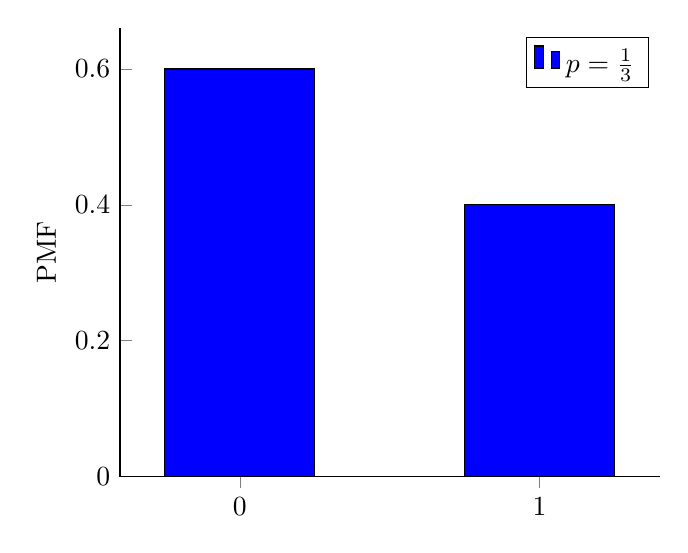
\begin{tikzpicture}
		\begin{axis}[every axis plot,
				ybar=0pt, bar width=0.5,
				ymin=0,
				xmin=-0.25, xmax=1.25,
				ylabel=PMF,
				axis x line*=bottom, % no box around the plot, only x and y axis
				axis y line*=left, % the * suppresses the arrow tips
				enlarge x limits=true, % extend the axes a bit
				xtick={0, 1}
			]

			\addplot [fill=blue] coordinates {
					(0, 0.6)
					(1, 0.4)};
			\addlegendentry{$p=\frac{1}{3}$}
		\end{axis}
	\end{tikzpicture}
\end{frame}

\subsubsection{Binomial}
\begin{frame}{Binomial}
	The binomial distribution describes an event in which the number of
	successes in a sequence $n$ independent experiments,
	each one making a yes--no question with probability of success $p$.
	Notice that Bernoulli distribution is a special case of the binomial
	distribution where $n=1$.
	\vfill
	The binomial distribution has two parameters and its notation is
	$\text{Binomial}(n, p)$ :
	\begin{vfilleditems}
		\item $n$ -- number of experiments
		\item $p$ -- probability of success
	\end{vfilleditems}
	\vfill
	Example: number of heads in five coin throws.
\end{frame}

\begin{frame}{Binomial}
	$$\text{Binomial}(n,p) = f(x, n, p) = \binom{n}{x}p^{x}(1-p)^{n-x} \text{ for $x \in \{0, 1, \dots, n\}$}$$
\end{frame}

\begin{frame}{Binomial}
	\centering
	\begin{tikzpicture}
		\begin{axis}[every axis plot,
				ybar=0pt, bar width=1,
				ylabel=PMF,
				ytick={0,0.05,...,0.15},
				samples at={0,...,40},
				axis x line*=bottom, % no box around the plot, only x and y axis
				axis y line*=left, % the * suppresses the arrow tips
				enlarge x limits=true, % extend the axes a bit
				y tick label style={/pgf/number format/.cd, fixed, fixed zerofill, precision=2}
			]

			\addplot [fill=blue, fill opacity=0.5] {binomial(40, 0.2)};
			\addlegendentry{$n=40, p=\frac{1}{5}$}
			\addplot [fill=red, fill opacity=0.5] {binomial(40, 0.5)};
			\addlegendentry{$n=40, p=\frac{1}{2}$}
		\end{axis}
	\end{tikzpicture}
\end{frame}

\subsubsection{Poisson}
\begin{frame}{Poisson}
	Poisson distribution describes the probability of a certain number of
	events occurring in a fixed time interval if these events
	occur with a constant mean rate which is known and independent since
	the time of last occurrence.
	Poisson distribution can also be used for number of events in other
	type of intervals, such as distance, area or volume.
	\vfill
	Poisson distribution has one parameter and its notation is $\text{Poisson}(\lambda)$:
	\begin{vfilleditems}
		\item $\lambda$ -- rate
	\end{vfilleditems}
	\vfill
	Example: number of e-mails that you receive daily or the number of the potholes you'll find in your commute.
\end{frame}

\begin{frame}{Poisson}
	$$\text{Poisson}(\lambda) = f(x, \lambda) = \frac{\lambda^x e^{-\lambda}}{x!} \text{ for $\lambda > 0$}$$
\end{frame}

\begin{frame}{Poisson}
	\centering
	\begin{tikzpicture}
		\begin{axis}[every axis plot,
				ybar=0pt, bar width=1,
				ylabel=PMF,
				samples at={0,...,8},
				axis x line*=bottom, % no box around the plot, only x and y axis
				axis y line*=left, % the * suppresses the arrow tips
				enlarge x limits=true, % extend the axes a bit
			]

			\addplot [fill=blue, fill opacity=0.5] {poisson(1)};
			\addlegendentry{$\lambda=2$}
			\addplot [fill=red, fill opacity=0.5] {poisson(4)};
			\addlegendentry{$\lambda=4$}
		\end{axis}
	\end{tikzpicture}
\end{frame}

\subsubsection{Negative Binomial}
\begin{frame}{Negative Binomial\footnote{
			any phenomena that can be modeles as a Poisson distribution can be
			modeled also as negative binomial distribution
			\parencite{gelman2013bayesian, gelman2020regression}.}}
	\small
	The binomial distribution describes an event in which the number of
	successes in a sequence $n$ independent experiments,
	each one making a yes--no question with probability of success $p$
	until $k$ successes.
	Notice that it becomes the Poisson distribution in the limit as $k \to \infty$.
	This makes it a robust option to replace a Poisson distribution to model
	phenomena with overdispersion
	(presence of greater variability in data than would be expected).
	\vfill \small
	The negative binomial has two parameters and its notation is
	$\text{Negative Binomial}(k, p)$:
	\begin{vfilleditems}
		\small
		\item $k$ -- number of successes
		\item $p$ -- probability of success
	\end{vfilleditems}
	\vfil \small
	Example: annual occurrence of tropical cyclones.
\end{frame}

\begin{frame}{Negative Binomial}
	$$
		\begin{aligned}
			\text{Negative Binomial}(k, p) & = f(x, k, p) & = \binom{x + k - 1}{k - 1}p^{x}(1-p)^{k} \\
			\\
			                               & ~            & \text{for $x \in \{0, 1, \dots, n\}$}
		\end{aligned}
	$$
\end{frame}

\begin{frame}{Negative Binomial}
	\centering
	\begin{tikzpicture}
		\begin{axis}[every axis plot,
				ybar=0pt, bar width=1,
				ylabel=PMF,
				samples at={0,...,8},
				axis x line*=bottom, % no box around the plot, only x and y axis
				axis y line*=left, % the * suppresses the arrow tips
				enlarge x limits=true, % extend the axes a bit
			]

			\addplot [fill=blue, fill opacity=0.5] {negativebinomial(1, 0.5)};
			\addlegendentry{$k=1, p=\frac{1}{2}$}
			\addplot [fill=red, fill opacity=0.5] {negativebinomial(5,0.5)};
			\addlegendentry{$k=5, p=\frac{1}{2}$}
		\end{axis}
	\end{tikzpicture}
\end{frame}

%--- Continuous ------------------------------------------------------%

\subsection{Continuous Distributions}
\begin{frame}
	\begin{defn}[Continuous Distributions]
		\small
		Continuous probability distributions are distributions which
		the results are values in a continuous real number line:
		$(-\infty, +\infty) \in \mathbb{R}$.
		In continuous probability distributions we call the probability
		of a distribution taking values as ``density''.
		Since we are referring to real numbers we cannot obtain the
		probability of a random variable $X$ taking exactly the value $x$.
		This will always be $0$, since we cannot specify the exact
		value of $x$. $x$ lies in the real number line, hence,
		we need to specify the probability of $X$ taking values in an
		interval $[a,b]$.
		The probability density function (PDF) is defined as:
		$$\text{PDF}(x) = P(a \leq X \leq b) = \int_a^b f(x) dx$$
	\end{defn}
\end{frame}

\subsubsection{Continuous Uniform}
\begin{frame}{Continuous Uniform}
	The continuous uniform distribution is a symmetric probability distribution
	in which an infinite number of value intervals are equally likely of being observable.
	Each one of the infinite $n$ intervals have probability $\frac{1}{n}$.
	\vfill
	The continuous uniform distribution has two parameters and its notation is $\text{Uniform}(a, b)$:
	\begin{vfilleditems}
		\item $a$ -- lower bound
		\item $b$ -- upper bound
	\end{vfilleditems}
\end{frame}

\begin{frame}{Continuous Uniform}
	$$\text{Uniform}(a,b) = f(x, a, b) = \frac{1}{b-a} \text{ for $a \leq x \leq b$ e $x \in [a, b]$}$$
\end{frame}

\begin{frame}{Continuous Uniform}
	\centering
	\begin{tikzpicture}
		\begin{axis}[every axis plot, line width=2pt,
				ylabel=PDF,
				domain=0:6,samples=200,
				axis x line*=bottom, % no box around the plot, only x and y axis
				axis y line*=left, % the * suppresses the arrow tips
				enlarge x limits=true, % extend the axes a bit
			]

			\addplot [blue] {continuousuniform(0, 6)};
			\addlegendentry{$a=0, b=6$}
		\end{axis}
	\end{tikzpicture}
\end{frame}

\subsubsection{Normal}
\begin{frame}{Normal}
	This distribution is generally used in social and natural sciences to
	represent continuous variables in which its underlying distribution are unknown.
	This assumption is due to the central limit theorem (CLT) that,
	under precise conditions, the mean of many samples (observations) of a
	random variable with finite mean and variance is itself a random variable
	which the underlying distribution converges to a normal distribution
	as the number of samples increases (as $n \to \infty$).
	\vfill
	Hence, physical quantities that we assume that are the sum of many
	independent processes (with measurement error) often have underlying
	distributions that are similar to normal distributions.
\end{frame}

\begin{frame}{Normal}
	The normal distribution has two parameters and its notation is
	$\text{Normal}(\mu, \sigma^2)$ or $\text{N}(\mu, \sigma^2)$:
	\begin{vfilleditems}
		\item $\mu$ -- mean of the distribution, and also median and mode
		\item $\sigma$ -- standard deviation\footnote{sometimes is also parameterized as variance $\sigma^2$.},
		a dispersion measure of how observations occur in relation from the mean
	\end{vfilleditems}
	\vfill
	Example: height, weight etc.
\end{frame}

\begin{frame}{Normal\footnote{
			see how the normal distribution was derived from the binomial
			distribution in the \hyperlink{appendixnormal}{backup slides}.}}
	$$\text{Normal}(\mu,\sigma) = f(x, \mu, \sigma) = \frac{1}{\sigma{\sqrt{2\pi }}}e^{-{\frac{1}{2}}\left({\frac {x-\mu }{\sigma }}\right)^{2}} \text{ for $\sigma > 0$}$$
\end{frame}

\begin{frame}{Normal}
	\centering
	\begin{tikzpicture}
		\begin{axis}[every axis plot, line width=2pt,
				ylabel=PDF,
				domain=-4:6,samples=200,
				axis x line*=bottom, % no box around the plot, only x and y axis
				axis y line*=left, % the * suppresses the arrow tips
				enlarge x limits=true, % extend the axes a bit
			]

			\addplot [blue] {gaussian(0, 1)};
			\addlegendentry{$\mu=0, \sigma=1$}
			\addplot [red] {gaussian(0, 2)};
			\addlegendentry{$\mu=0, \sigma=2$}
			\addplot [yellow] {gaussian(2, 1)};
			\addlegendentry{$\mu=2, \sigma=1$}
		\end{axis}
	\end{tikzpicture}
\end{frame}

\subsubsection{Log-Normal}
\begin{frame}{Log-Normal}
	The log-normal distribution is a continuous probability distribution of a
	random variable which its natural logarithm is distributed as a normal distribution.
	Thus, if the natural logarithm a random variable $X$, $\ln(X)$, is distributed
	as a normal distribution, then $Y = \ln(X)$ is normally distributed and
	$X$ is log-normally distributed.
	\vfill
	A a log-normal random variable only takes positive real values.
	It is a convenient and useful model for measurements in exact and engineering
	sciences, as well as in biomedical, economical and other sciences.
	For example, energy, concentrations, length, financial returns and other measurements.
	\vfill
	A log-normal process is the statistical realization of a multiplicative
	product of many independent positive random variables.
\end{frame}

\begin{frame}{Log-Normal}
	The log-normal distribution has two parameters and its notation is
	$\text{Log-Normal}(\mu, \sigma^2)$:
	\begin{vfilleditems}
		\item $\mu$ -- mean of the distribution's natural logarithm
		\item $\sigma$ -- square root of the variance of the distribution's natural logarithm
	\end{vfilleditems}
\end{frame}

\begin{frame}{Log-Normal}
	$$\text{Log-Normal}(\mu,\sigma) = f(x, \mu, \sigma) = \frac{1}{x \sigma{\sqrt{2\pi}}}e^{-\left({\frac {(\ln(x)-\mu)^2}{2 \sigma^2 }}\right)} \text{ for $\sigma > 0$}$$
\end{frame}

\begin{frame}{Log-Normal}
	\centering
	\begin{tikzpicture}
		\begin{axis}[every axis plot, line width=2pt,
				ylabel=PDF,
				domain=0:5,samples=200,
				axis x line*=bottom, % no box around the plot, only x and y axis
				axis y line*=left, % the * suppresses the arrow tips
				enlarge x limits=true, % extend the axes a bit
			]

			\addplot [blue] {lognormal(0, 0.25)};
			\addlegendentry{$\mu=0, \sigma=\frac{1}{4}$}
			\addplot [red] {lognormal(0, 1)};
			\addlegendentry{$\mu=0, \sigma=1$}
			\addplot [yellow] {lognormal(1, 1)};
			\addlegendentry{$\mu=1, \sigma=1$}
		\end{axis}
	\end{tikzpicture}
\end{frame}

\subsubsection{Exponential}
\begin{frame}{Exponential}
	The exponential distribution is the probability distribution of the time
	between events that occurs in a continuos manner, are independent,
	and have constant mean rate of occurrence.
	\vfill
	The exponential distribution has one parameter and its notation is
	$\text{Exponential}(\lambda)$:
	\begin{vfilleditems}
		\item $\lambda$ -- rate
	\end{vfilleditems}
	\vfill
	Example: How long until the next earthquake or how long until the next bus arrives.
\end{frame}

\begin{frame}{Exponential}
	$$\text{Exp}(\lambda) = f(x, \lambda) = \lambda e^{-\lambda x} \text{ for $\lambda > 0$}$$
\end{frame}

\begin{frame}{Exponential}
	\centering
	\begin{tikzpicture}
		\begin{axis}[every axis plot, line width=2pt,
				ylabel=PDF,
				domain=0:5,samples=200,
				axis x line*=bottom, % no box around the plot, only x and y axis
				axis y line*=left, % the * suppresses the arrow tips
				enlarge x limits=true, % extend the axes a bit
			]

			\addplot [blue] {exponential(0.5)};
			\addlegendentry{$\lambda=\frac{1}{2}$}
			\addplot [red] {exponential(1)};
			\addlegendentry{$\lambda=1$}
			\addplot [yellow] {exponential(2)};
			\addlegendentry{$\lambda=2$}
		\end{axis}
	\end{tikzpicture}
\end{frame}

\subsubsection{Gamma}
\begin{frame}{Gamma}
	The gammma distribution is a long-tailed distribution with support only for positive real numbers.
	\vfill
	The gamma distribution has two parameters and its notation is
	$\text{Gamma}(\alpha, \theta)$:
	\begin{vfilleditems}
		\item $\alpha$ -- shape parameter
		\item $\theta$ -- rate parameter
	\end{vfilleditems}
	\vfill
	Example: Any waiting time can be modelled with a gamma distribution.
\end{frame}

\begin{frame}{Gamma}
	$$\text{Gamma}(\alpha, \theta) = f(x, \alpha, \theta) = \frac{x^{\alpha-1} e^{-x/\theta}}{\Gamma(\alpha) \theta^\alpha} \text{ for $x,\alpha,\theta > 0$}$$
\end{frame}

\begin{frame}{Gamma}
	\centering
	\begin{tikzpicture}
		\begin{axis}[every axis plot, line width=2pt,
				ylabel=PDF,
				domain=0:14,samples=200,
				axis x line*=bottom, % no box around the plot, only x and y axis
				axis y line*=left, % the * suppresses the arrow tips
				enlarge x limits=true, % extend the axes a bit
			]

			\addplot [blue] {gammadist(1, 2)};
			\addlegendentry{$\alpha=1, \theta=2$}
			\addplot [red] {gammadist(2, 2)};
			\addlegendentry{$\alpha=2, \theta=2$}
			\addplot [yellow] {gammadist(3, 1)};
			\addlegendentry{$\alpha=3, \theta=\frac{1}{2}$}
		\end{axis}
	\end{tikzpicture}
\end{frame}

\subsubsection{Student's $t$}
\begin{frame}{Student's $t$}
	Student's $t$ distribution arises by estimating the mean of a normally-distributed
	population in situations where the sample size is small and the standard
	deviation is known\footnote{this is where the ubiquitous Student's $t$ test.}.
	\vfill
	If we take a sample of $n$ observations from a normal distribution,
	then Student's $t$ distribution with $\nu = n-1$ degrees of freedom can
	be defined as the distribution of the location of the sample mean
	in relation to the true mean, divided by the sample's standard deviation,
	after multiplying by the scaling term $\sqrt{n}$.
	\vfill
	Student's $t$ distribution is symmetric and in a bell-shape,
	like the normal distribution, but with long tails,
	which means that has more chance to produce values far away from its mean.
\end{frame}

\begin{frame}{Student's $t$}
	Student's $t$ distribution has one parameter and its notation is
	$\text{Student}(\nu)$:
	\begin{vfilleditems}
		\item $\nu$ -- degrees of freedom, controls how much it resembles a normal distribution
	\end{vfilleditems}
	\vfill
	Example: a dataset full of outliers.
\end{frame}

\begin{frame}{Student's $t$}
	$$\text{Student}(\nu) = f(x, \nu) = \frac{\Gamma \left(\frac{\nu+1}{2} \right)} {\sqrt{\nu\pi}\,\Gamma \left(\frac{\nu}{2} \right)} \left(1+\frac{x^2}{\nu} \right)^{-\frac{\nu+1}{2}} \text{ for $\nu \geq 1$}$$
\end{frame}

\begin{frame}{Student's $t$}
	\centering
	\begin{tikzpicture}
		\begin{axis}[every axis plot, line width=2pt,
				ylabel=PDF,
				domain=-4:4,samples=200,
				axis x line*=bottom, % no box around the plot, only x and y axis
				axis y line*=left, % the * suppresses the arrow tips
				enlarge x limits=true, % extend the axes a bit
			]

			\addplot [blue] {student(1)};
			\addlegendentry{$\nu=1$}
			\addplot [red] {student(3)};
			\addlegendentry{$\nu=3$}
			\addplot [yellow] {student(30)};
			\addlegendentry{$\nu=30$}
		\end{axis}
	\end{tikzpicture}
\end{frame}

\subsubsection{Cauchy}
\begin{frame}{Cauchy}
	The Cauchy distribution is bell-shaped distribution and a special case for Student's $t$ with $\nu=1$.
	\vfill
	But, differently than Student's $t$, the Cauchy distribution has two parameters and its notation is
	$\text{Gamma}(\alpha, \theta)$:
	\begin{vfilleditems}
		\item $\mu$ -- location parameter
		\item $\sigma$ -- scale parameter
	\end{vfilleditems}
	\vfill
	Example: a dataset full of outliers.
\end{frame}

\begin{frame}{Cauchy}
	$$\text{Cauchy}(\mu, \sigma) = \frac{1}{\pi \sigma \left(1 + \left(\frac{x - \mu}{\sigma} \right)^2 \right)} \text{ for $\sigma \geq 0$}$$
\end{frame}

\begin{frame}{Cauchy}
	\centering
	\begin{tikzpicture}
		\begin{axis}[every axis plot, line width=2pt,
				ylabel=PDF,
				domain=-4:4,samples=200,
				axis x line*=bottom, % no box around the plot, only x and y axis
				axis y line*=left, % the * suppresses the arrow tips
				enlarge x limits=true, % extend the axes a bit
			]

			\addplot [blue] {cauchy(0, 1)};
			\addlegendentry{$\mu=0, \sigma=1$}
			\addplot [red] {cauchy(0, 0.5)};
			\addlegendentry{$\mu=0, \sigma=\frac{1}{2}$}
			\addplot [yellow] {cauchy(-2, 1)};
			\addlegendentry{$\mu=-2, \sigma=1$}
		\end{axis}
	\end{tikzpicture}
\end{frame}

\subsubsection{Beta}
\begin{frame}{Beta}
	The beta distribution is a natural choice to model anything that is
	restricted to values between $0$ e $1$.
	Hence, it is a good candidate to model probabilities and proportions.
	\vfill
	The beta distribution has two parameters and its notations is
	$\text{Beta} (\alpha, \beta)$:
	\begin{vfilleditems}
		\item $\alpha$ or sometimes $a$ -- shape parameter,
		controls how much the shape is shifted towards $1$
		\item $\beta$ or sometimes $b$ -- shape parameter,
		controls how much the shape is shifted towards $0$
	\end{vfilleditems}
	\vfill
	Example: A basketball player that has already scored 5 free throws and
	missed 3 in a total of 8 attempts -- $\text{Beta}(3, 5)$
\end{frame}

\begin{frame}{Beta}
	$$\text{Beta} (\alpha, \beta) = f(x, \alpha, \beta) \frac{x^{\alpha-1}(1-x)^{\beta-1}} {\frac{\Gamma (\alpha )\Gamma (\beta )}{\Gamma (\alpha +\beta )}} \text{ for $\alpha,\beta > 0$ and $x \in [0, 1]$}$$
\end{frame}

\begin{frame}{Beta}
	\centering
	\begin{tikzpicture}
		\begin{axis}[every axis plot, line width=2pt,
				ylabel=PDF,
				domain=0:1,samples=200,
				axis x line*=bottom, % no box around the plot, only x and y axis
				axis y line*=left, % the * suppresses the arrow tips
				enlarge x limits=true, % extend the axes a bit
			]

			\addplot [blue] {beta(1,1)};
			\addlegendentry{$\alpha=\beta=1$}
			\addplot [red] {beta(3,2)};
			\addlegendentry{$\alpha=3,\beta=2$}
			\addplot [yellow] {beta(2,3)};
			\addlegendentry{$\alpha=2,\beta=3$}
		\end{axis}
	\end{tikzpicture}
\end{frame}
